\chapter{Bookstore UML Modeling \\
  \small{\textit{-- Evan Ciok, Sophia DiCuffa, Carson McManus}}
  \index{Chapter!labone}
  \index{Lab One}
  \label{Chapter::LabOne}}

% Add a section and label it so that we can reference it later
\section{Bookstore UML Modeling \label{Section::LabOne}}

\begin{figure}
  \centering
  \scalebox{0.3}{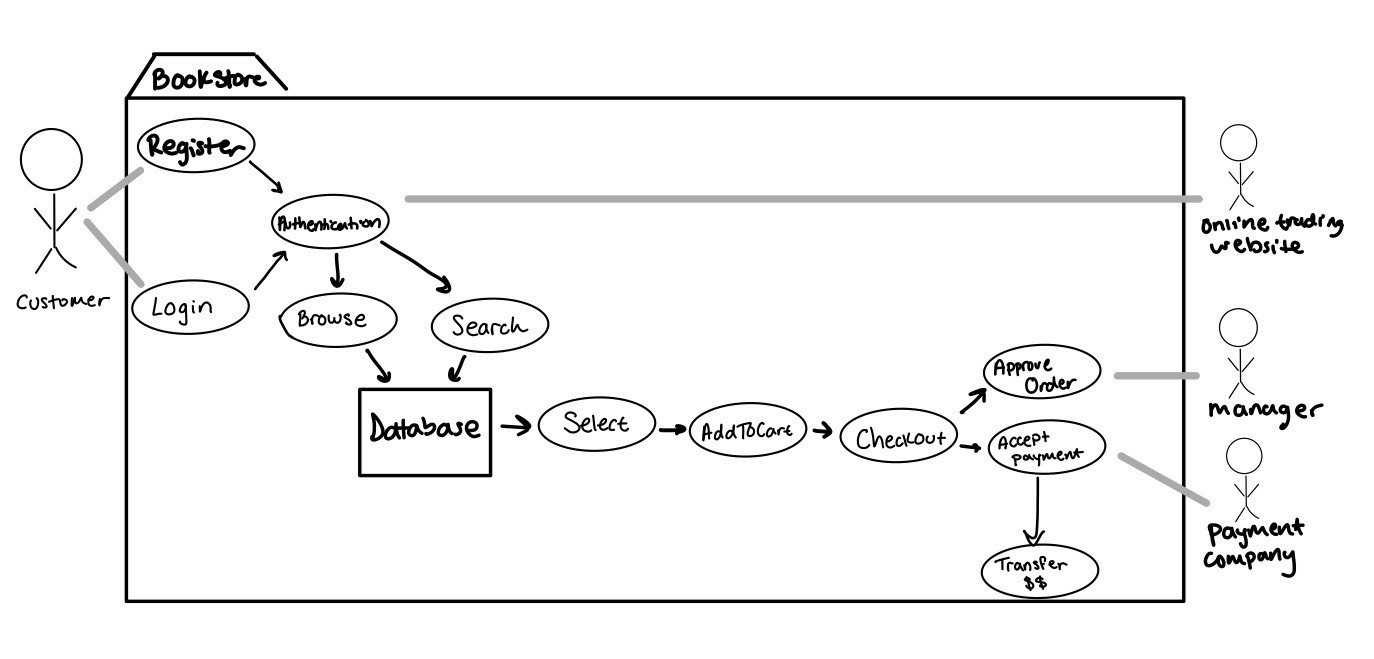
\includegraphics{Figures/bookstore/usecase.jpg}}
  \caption{\label{Figure::bookstoreUseCase} A use-case diagram for the e-Bookstore system that supports the list of functions shown above.}
\end{figure}

\begin{figure}
  \centering
  \scalebox{0.25}{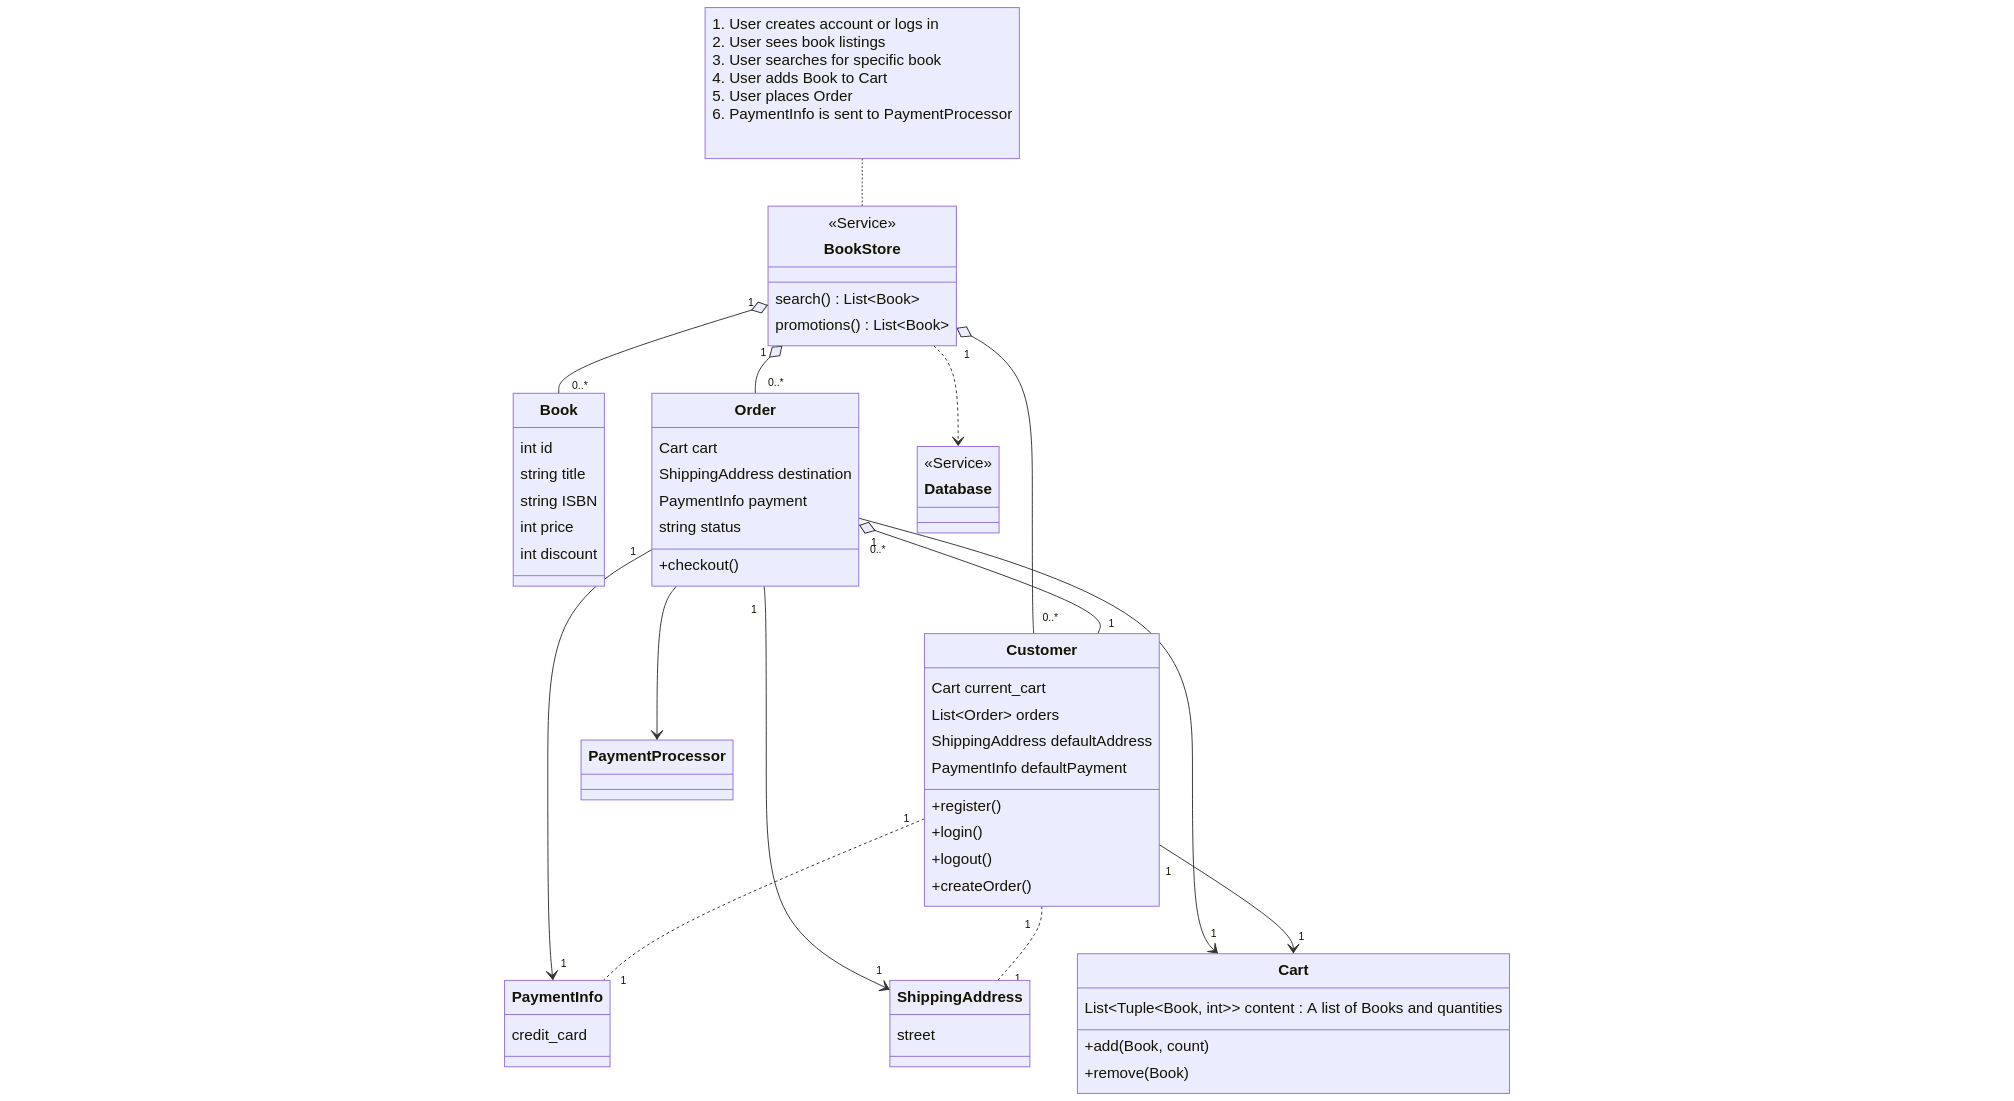
\includegraphics{Figures/bookstore/uml.png}}
  \caption{\label{Figure::bookstoreUML} A class diagram for the e-Bookstore system that illustrates the choices of the main classes and
    appropriate relationships among them.}
\end{figure}

\begin{figure}
  \centering
  \scalebox{0.25}{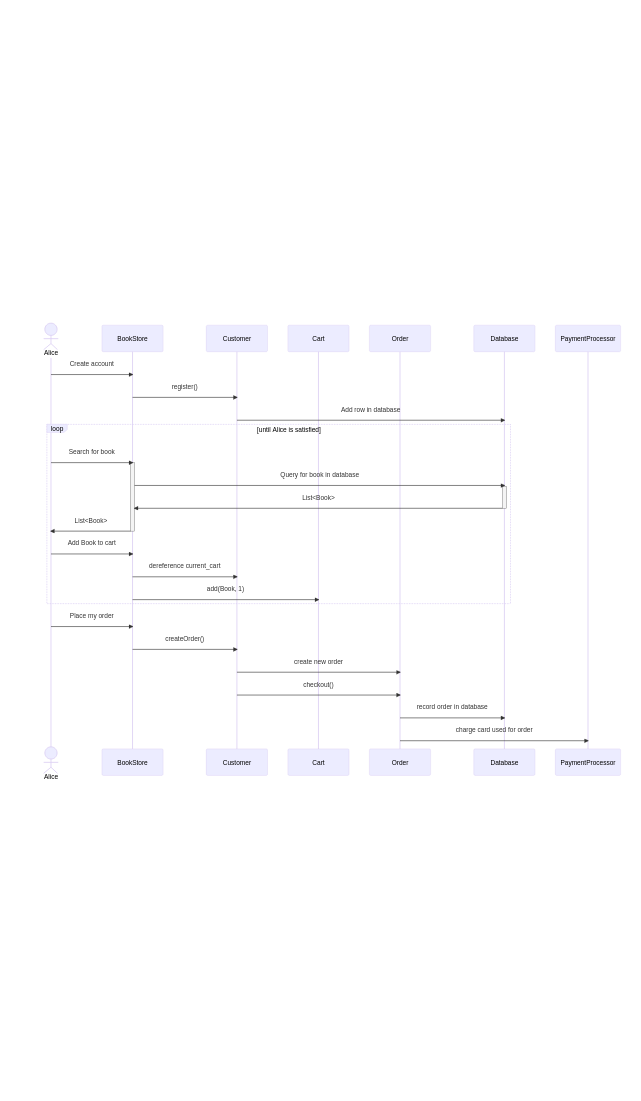
\includegraphics{Figures/bookstore/sequence.png}}
  \caption{\label{Figure::bookstoreSequence} A sequence diagram for the e-Bookstore system that illustrates the choices of the main classes and
    appropriate relationships among them.}
\end{figure}